\item {\bf Double Descent on Linear Models}

% {\bf Note:} This question may require knowledge on double descent that is covered on Wed of Week 5. 

In this problem, you will empirically observe the sample-wise double descent phenomenon. That is, the validation losses of some learning algorithms or estimators do not monotonically decrease as we have more training examples, but instead have a curve with two U-shaped parts. The double descent phenomenon can be observed even for simple linear models. In this question, we consider the following setup. Let $\{(x^{(i)},y^{(i)})\}_{i=1}^{n}$ be the training dataset. Let $X\in\R^{n\times d}$ be the matrix representing the inputs (i.e., the $i$-th row of $X$ corresponds to $x^{(i)})$), and $\vec{y}\in\R^{n}$ the vector representing the labels (i.e., the $i$-th row of $\vec{y}$ corresponds to $y^{(i)})$):
$$
X=
\begin{bmatrix}
	- & x^{(1)} & - \\
	- & x^{(2)} & - \\
	\vdots & \vdots & \vdots\\
	- & x^{(n)} & - 
\end{bmatrix},\qquad
\vec{y}=
\begin{bmatrix}
	y^{(1)} \\
	y^{(2)}\\
	\vdots\\
	y^{(n)}
\end{bmatrix}.
$$
Similarly, we use $X_v\in \R^{m\times d}, \vec{y}_v\in \R^{m}$ to represent the validation dataset, where $m$ is the size of the validation dataset. We assume that the data are generated with $d=500$. 

In this question, we consider \emph{regularized} linear regression. For a regularization level $\lambda\ge 0$, define the regularized cost function $$J_\lambda(\beta)=\frac{1}{2}\|X\beta-\vec{y}\|_2^2+\frac{\lambda}{2}\|\beta\|_2^2,$$ and its minimizer $\hat{\beta}_\lambda=\arg\min_{\beta\in \R^{d}}J_\lambda(\beta).$

\begin{enumerate}
  \item \points{4a}
\textbf{Derive closed-form solution.}

In this question, we derive the closed-form solution of $\hat{\beta}_\lambda.$ \textbf{Prove} that when $\lambda>0$, 
\begin{equation}
	\hat{\beta}_\lambda=(X^\top X+\lambda I_{d\times d})^{-1}X^\top \vec{y} \label{equ:sol}
\end{equation} (recall that $I_{d\times d}\in \R^{d\times d}$ is the identity matrix.)

\textbf{Note:} $\lambda=0$ is a special case here. When $\lambda=0$, $(X^\top X+\lambda I_{d\times d})$ could be singular. Therefore, there might be more than one solutions that minimize $J_0(\beta)$. In this case, we define $\hat{\beta}_0$ in the following way:
\begin{align}
	\hat{\beta}_0=(X^\top X)^{+}X^\top \vec{y}.
\end{align}
where $(X^\top X)^{+}$ denotes the \href{https://en.wikipedia.org/wiki/Moore-Penrose_inverse}{Moore-Penrose pseudo-inverse} of $X^\top X$. You don't need to prove the case when $\lambda=0$, but this definition is useful in the following sub-questions. 

  \item \points{4b}
\textbf{The double descent phenomenon for unregularized models}

In this question, you will empirically observe the double descent phenomenon.You are given $13$ training datasets of sample sizes $n  = 200, 250, \dots, 750$, and $800$, and a validation dataset, located at
\begin{itemize}
	\item \texttt{src-doubledescent/train200.csv}, \texttt{train250.csv}, etc.
	\item \texttt{src-doubledescent/validation.csv}
\end{itemize} 

For each training dataset $(X, \vec{y})$, compute the corresponding $\hat{\beta}_0$, and evaluate the mean squared error (MSE) of $\hat{\beta}_0$ on the validation dataset. The MSE for your estimators $\hat{\beta}$ on a validation dataset $(X_v, \vec{y}_v)$ of size $m$ is defined as: $$\text{MSE}(\hat{\beta}) = \frac{1}{2m} \|X_v \hat{\beta}-\vec{y}_v\|^2_2.$$


Complete the \texttt{regression} method of \texttt{src-doubledescent/submission.py} which takes in a training file and a validation file, and computes $\hat{\beta}_0$. You can use \texttt{numpy.linalg.pinv} to compute the pseudo-inverse.


The output plot should look similar to the following (no plot submission is required):

\begin{figure}[H]
	\centering
	\vspace{-2mm}
	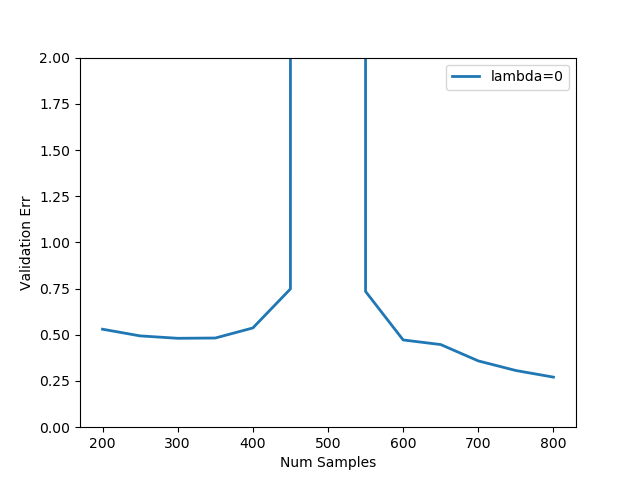
\includegraphics[width=0.65\linewidth]{04-doubledescent/unreg.png}
	\caption{Num of samples vs. validation error.}
	\centering
\end{figure}

The x-axis is the size of the training dataset (from 200 to 800); the y-axis is the MSE on the validation dataset. You should observe that the validation error increases and then decreases as we increase the sample size.

\textbf{Note:} When $n\approx d$, the test MSE could be very large. For better visualization, we let the if the test MSE goes out of scope in the plot for some points.

  \item \points{4c}
\textbf{Duble descent phenomenon and the effect of regularization. }

In this question, we will show that regularization mitigates the double descent phenomenon for linear regression. We will use the same datasets as specified in sub-question (b). Now consider using various regularization strengths. For $\lambda\in \{0, 1, 5, 10, 50, 250, 500, 1000\}$, you will compute the minimizer of $J_\lambda(\beta).$ 

Complete the \texttt{ridge\_regression} method of \texttt{src-doubledescent/submission.py} which takes in a training file and a validation file, computes the $\hat{\beta}_\lambda$ that minimizes the training objective under different regularization strengths, and returns a list of validation errors (one for each choice of $\lambda$).



The output plot should look similar to the following (no plot submission is required):

\begin{figure}[H]
    \centering
    \vspace{-2mm}
    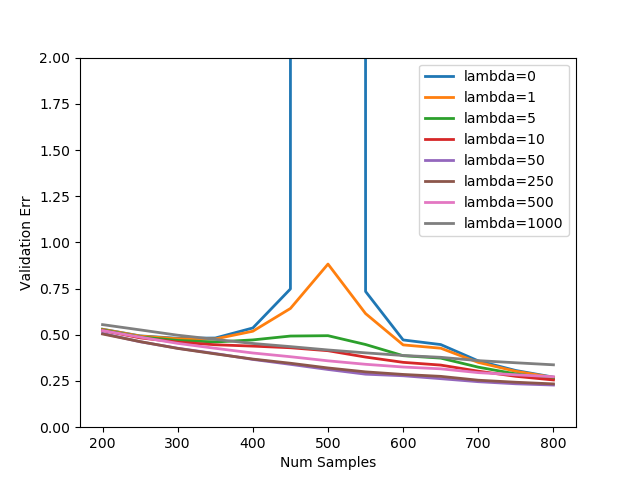
\includegraphics[width=0.65\linewidth]{04-doubledescent/reg.png}
    \caption{Num of samples vs. validation error for different regularization strengths}
    \centering
\end{figure}


The x-axis is the size of the training dataset (from 200 to 800); the y-axis is the MSE on the validation dataset.


You should observe that for some small $\lambda$'s, the validation error may increase and then decrease as we increase the sample size. However, double descent does not occur for a relatively large $\lambda$. 


\textbf{Remark:} If you want to learn more about the double descent phenomenon and the effect of regularization, you can start with this paper \href{https://arxiv.org/abs/2003.01897}{Nakkiran, et al. 2020}.
\end{enumerate}
